\documentclass[tikz,border=2pt]{standalone}

\usepackage{tikz}
\usetikzlibrary{arrows.meta}

\begin{document}

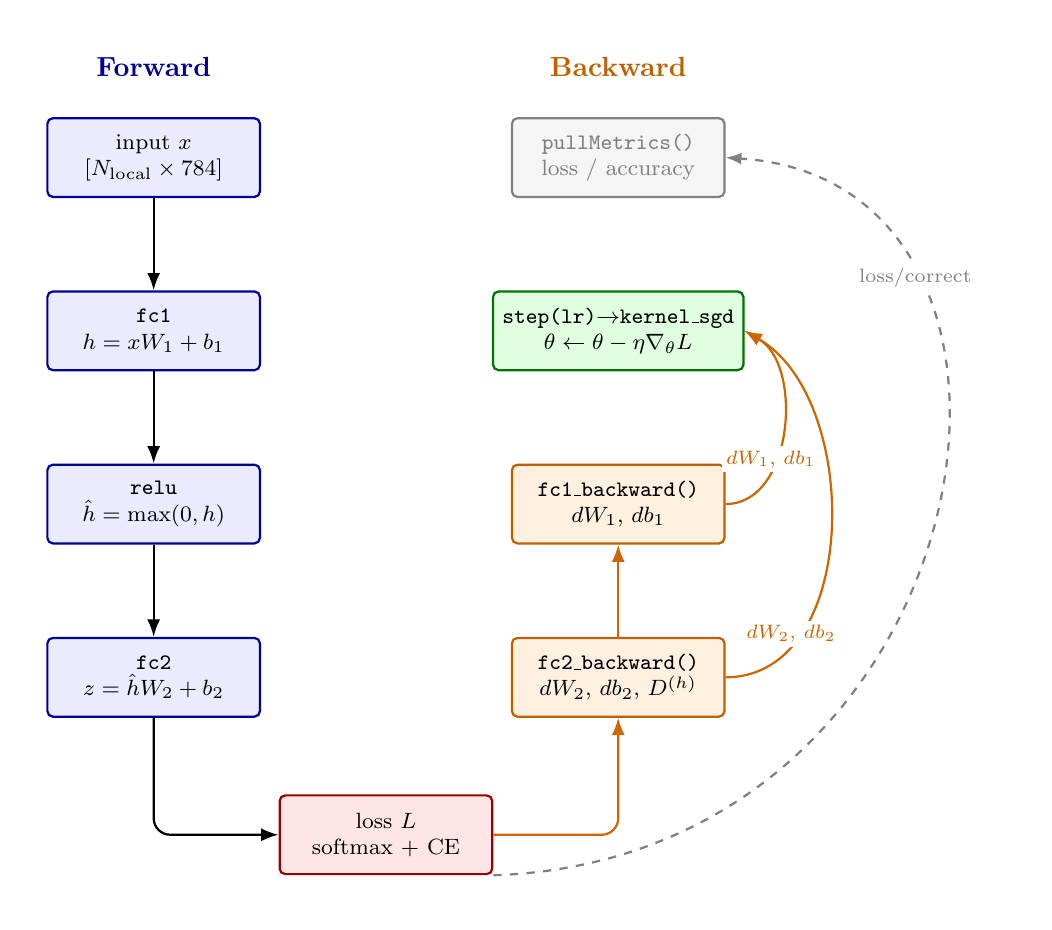
\begin{tikzpicture}[
    font=\footnotesize,
    fwd/.style={draw=blue!60!black, thick, rounded corners=2pt, fill=blue!8,
                minimum width=2.7cm, minimum height=1.0cm, align=center},
    lossS/.style={draw=red!60!black, thick, rounded corners=2pt, fill=red!10,
                  minimum width=2.7cm, minimum height=1.0cm, align=center},
    bwd/.style={draw=orange!75!black, thick, rounded corners=2pt, fill=orange!12,
                minimum width=2.7cm, minimum height=1.0cm, align=center},
    stepS/.style={draw=green!45!black, thick, rounded corners=2pt, fill=green!12,
                  minimum width=2.7cm, minimum height=1.0cm, align=center},
    metr/.style={draw=gray, thick, rounded corners=2pt, fill=gray!8, text=gray,
                 minimum width=2.7cm, minimum height=1.0cm, align=center},
    arr/.style={-{Latex[length=2.2mm]}, thick},
    barr/.style={-{Latex[length=2.2mm]}, thick, orange!80!black},
    garr/.style={-{Latex[length=2mm]}, thick, gray, dashed},
    lab/.style={font=\scriptsize, inner sep=1.5pt, align=center, fill=white,
                fill opacity=1, text opacity=1}
]
    \node[font=\normalsize\bfseries, blue!60!black] at (0,9.35) {Forward};
    \node[font=\normalsize\bfseries, orange!75!black] at (5.9,9.35) {Backward};

    \node[fwd] (x) at (0,8.2) {input $x$\\ $[N_{\mathrm{local}} \times 784]$};
    \node[fwd] (fc1) at (0,6.0) {\texttt{fc1}\\ $h = x W_1 + b_1$};
    \node[fwd] (relu) at (0,3.8) {\texttt{relu}\\ $\hat{h} = \max(0,h)$};
    \node[fwd] (fc2) at (0,1.6) {\texttt{fc2}\\ $z = \hat{h} W_2 + b_2$};

    \node[lossS] (loss) at (2.95,-0.4) {loss $L$\\ softmax + CE};

    \node[bwd] (fc2b) at (5.9,1.6)
        {\texttt{fc2\_backward()}\\ $dW_2,\,db_2,\,D^{(h)}$};
    \node[bwd] (fc1b) at (5.9,3.8)
        {\texttt{fc1\_backward()}\\ $dW_1,\,db_1$};
    \node[stepS] (step) at (5.9,6.0)
        {\texttt{step(lr)}$\rightarrow$\texttt{kernel\_sgd}\\
         $\theta \leftarrow \theta - \eta \nabla_{\theta}L$};
    \node[metr] (pull) at (5.9,8.2)
        {\texttt{pullMetrics()}\\ loss / accuracy};

    \draw[arr] (x) -- (fc1);
    \draw[arr] (fc1) -- (relu);
    \draw[arr] (relu) -- (fc2);
    \draw[arr,rounded corners=6pt] (fc2.south) |- (loss.west);

    \draw[barr,rounded corners=6pt] (loss.east) -| (fc2b.south);
    \draw[barr] (fc2b) -- (fc1b);

    \draw[barr] (fc2b.east) to[out=0,in=-30]
        node[lab,above,pos=0.2] {$dW_2,\,db_2$} (step.east);
    \draw[barr] (fc1b.east) to[out=0,in=-30]
        node[lab,above,pos=0.3] {$dW_1,\,db_1$} (step.east);

    \draw[garr] (loss.south east) .. controls +(6.3,0.2) and +(4.7,-0.3) ..
        node[lab,pos=0.75,text=gray] {loss/correct} (pull.east);

    \pgfresetboundingbox
    \path[use as bounding box] (-1.6,-1.25) rectangle (11.05,9.85);
\end{tikzpicture}

\end{document}
